%\addcontentsline{toc}{chapter}{}
\chapter{MySql/Mariadb}
\stepcounter{chapter}
MariaDB es una bifurcación de MySQL impulsada por la comunidad que Monty inició en 2009 Widenius, el autor original de MySQL, después de que Oracle adquiriera el antiguo proyecto.
La primera versión de MariaDB se basó en MySQL 5.1 y las mejoras a El código base de MySQL se fusiona regularmente en el proyecto MariaDB. Otras características
también se fusionan desde Percona Server\footnote{Percona Server for MySQL® es un reemplazo gratuito, totalmente compatible, mejorado y de código abierto para cualquier base de datos MySQL. Proporciona un rendimiento superior, escalabilidad e instrumentación.}, otra bifurcación que es muy similar a la producto principal.

Se utiliza el la siguiente versión:
\begin{verbatim}
Welcome to the MariaDB monitor.  Commands end with ; or \g.
Your MariaDB connection id is 31
Server version: 10.5.15-MariaDB-0+deb11u1 Debian 11
Copyright (c) 2000, 2018, Oracle, MariaDB Corporation Ab and others.
\end{verbatim}

\begin{figure}[h]
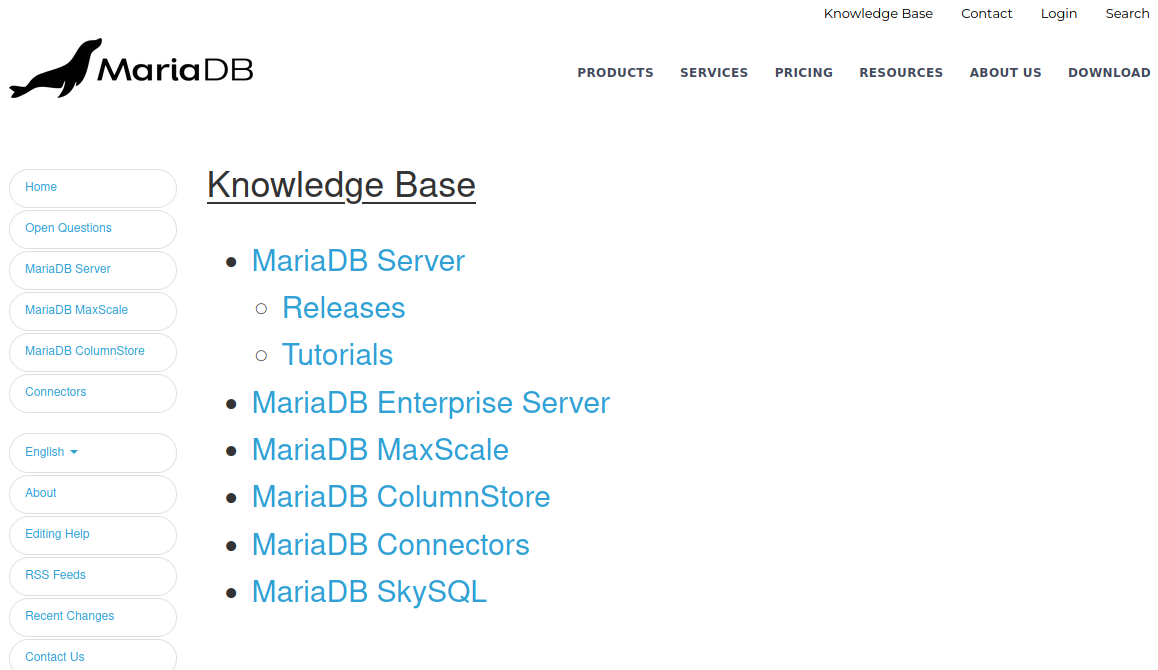
\includegraphics[scale=0.5]{images/maria1}
\end{figure}

